\section{Déroulement du Jeu}



\subsection{Initialisation }

\indent Cette phase se déroule au début du jeu avant le premier tour de jeu et après le chargement des joueurs. Elle consiste principalement en l'initialisation de plateau de jeu avec des tuiles "fantômes" :NONE, l'ajout de la tuile de départ et l'initialisation des édifices. Ainsi que la création et le mélange du deck des tuiles qui serviront pour la partie.

\subsection{Dynamique du jeu}
\indent La phase JOUER correspond à :
\\

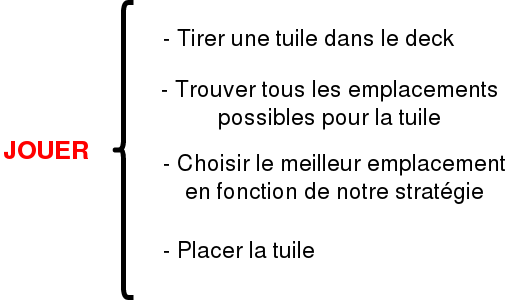
\includegraphics[scale=0.5]{Jouer.png}

Les fonctions "tirer une carte" et "la placer dans le boardgame" se font directement grâce à la $structure$ $boardgame$. \\


\begin{algorithm}[!h]
\caption{ Trouver un Emplacement }
\begin{algorithmic} [!h]
\REQUIRE  P : Plateau de jeux
\REQUIRE  $T_p $ : tuile pioché
\STATE $Lst_{possible} \leftarrow Lst_{vide}()$
\FOR{$T_i \in P$}
\IF{$\exists Emplacement \in Voisinage(T_i)$}
\STATE $Ajout(Lst_{possible},Emplacement)$
\ENDIF
\ENDFOR
\end{algorithmic}
\end{algorithm}

la complexité de cette algorithme est $\mathcal{O}(n^2)$ (n=Nombre\_Cartes)

Pour trouver un emplacement possible il faut :
\begin{itemize}
    \item trouver toutes les tuiles qui ont des emplacements libres
    \item vérifier que le coté coïncide avec notre tuile piochée
    \item vérifier que les autres cotés s'insèrent avec leur voisin
    \item et cela pour les 4 orientations possibles de la tuile piochée.
\end{itemize}

\vspace{0.5cm}

\begin{minipage}{0.5\linewidth}
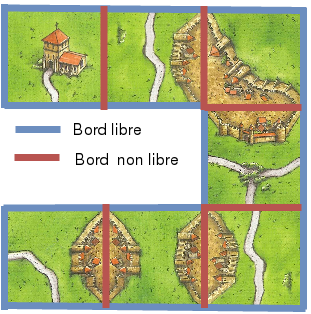
\includegraphics[scale=0.5]{BordLibre.png}
\end{minipage}\hfill
\begin{minipage}{0.5\linewidth}
Dans les cas où les bords sont non libres, l'algorithme va simplement continuer à se propager dans le plateau de jeu. Et ce, jusqu'à trouver un bord libre pour procéder après aux tests pour savoir si la tuile peut être posée ou non.
\end{minipage}

\begin{minipage}{0.5\linewidth}
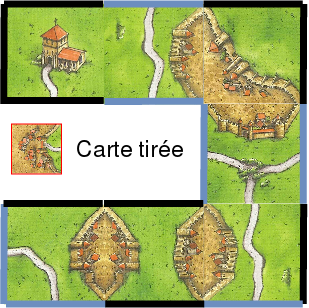
\includegraphics[scale=0.5]{CotePossible.png} 
\end{minipage}\hfill
\begin{minipage}{0.5\linewidth}
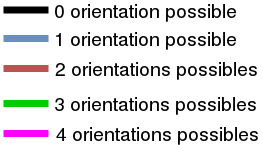
\includegraphics[scale=0.5]{CodeCouleur.png}
\end{minipage}

\vspace{1cm}

\begin{minipage}{0.7\linewidth}
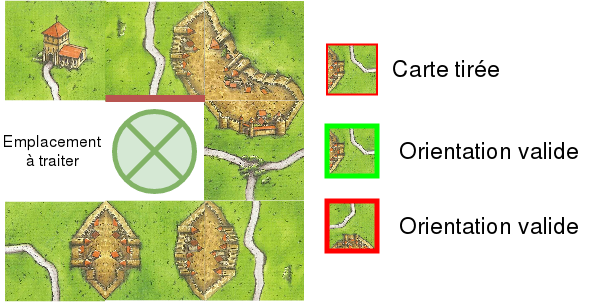
\includegraphics[scale=0.5]{ChoixOrientation.png}
\end{minipage}\hfill
\begin{minipage}{0.3\linewidth}
Dans cette situation, on se demande si l'on peut placer la tuile à partir du rebord en rouge (deux orientations sont donc possibles). En étudiant la topographie de la carte, l'algorithme va remarquer qu'une seule des deux orientations possibles\hspace{0.2cm} est\hspace{0.2cm} valide.\hspace{0.2cm} En effet, 
\end{minipage}

\begin{minipage}{1\linewidth}
     l'orientation typée "rouge" est invalide. Elle impose qu'un milieu de ville soit directement en contact avec un milieu de champ. Seule la verte sera donc retenue parmi les choix possibles. 
\end{minipage}
\hspace{1cm}
\newline
Enfin, la sélection de la position finale de la tuile demande de mettre en place une stratégie. Celle-ci devra prendre en compte les coups joués précédemment, la position et l'orientation des tuiles et surtout le positionnement des pions. Ce qui est simplifié par nos structures de données car elles permettent d' accéder directement aux édifices.On peut différencier 3 types de stratégies  : 
    
    \vspace{0.5cm}
    
\textbf{Renforcement}

Il s'agit de la stratégie de base qui consiste à continuer à achever les champs, villes, abbayes et routes et d'essayer de maximiser les points qu'elles rapportent (maximiser leur taille). Cette stratégie ignore donc les autres joueurs pour se concentrer sur ses propres édifices.
\newline

 \textbf{Bloqueur}

C'est la stratégie inverse, elle consiste à se concentrer principalement sur les édifices et à rajouter des tuiles qui bloquent/compliquent leur développement.

Exemple :

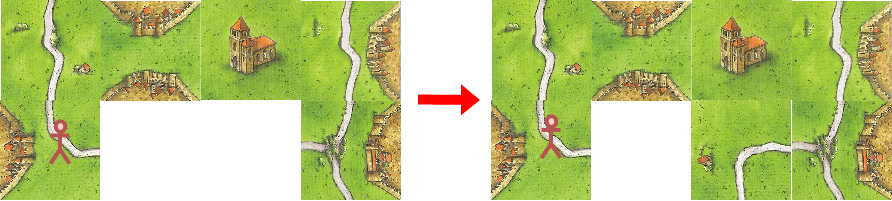
\includegraphics[scale=0.5]{Bloquer.png}

 Ici, le joueur aura beaucoup de mal à finir sa route à moins d'obtenir la seule tuile qui va à l'emplacement suivant.
 
 \vspace{0.5cm}
 
 \textbf{Parasite}

Cette stratégie prend le contre pied de la précédente. Elle se concentre aussi sur les autres joueurs mais essaye plutôt de s'incruster dans les édifices des autres joueurs afin de gagner le même nombre de points que eux.

Par exemple :

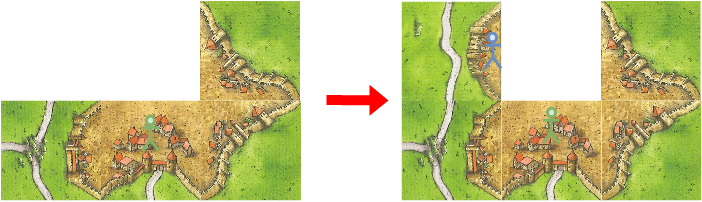
\includegraphics[scale=0.5]{Parasite.png}

Le joueur vert est en train de construire une grande ville qui va lui rapporter énormément de points. Cependant, le joueur bleu, en posant sa tuile juste à coté, se donne la possibilité de se raccrocher à la ville de son voisin. Ainsi avec une tuile le joueur bleu a marqué autant de points que le joueur vert avec toutes ses tuiles. \newline


On finit par insérer la tuile sur le plateau, avec le pion placé au milieu choisi, ce qui se fait facilement grâce à nos structures : soit le milieu n'appartient à aucune structure et on peut le mettre, soit il appartient à une structure et on ne peut pas placer de pion.

\subsection{La mise à jour}

Cette phase est la plus importante, il faut mettre à jour nos structures de données après l'ajout d'une tuile. En effet, nos structures contiennent beaucoup d'informations ce qui nous permet de réduire notre complexité en temps et de simplifier le calcul des points. Elle se fait suivant les étapes :

\vspace{0.5cm}


\includegraphics[scale=0.75]{Update.png}

\vspace{0.5cm}
\subsubsection{La mise à jour des routes}

\vspace{0.5cm}

\begin{algorithm}[!h]
\caption{ Update Road}
\begin{algorithmic} [!h]
\REQUIRE  B : boardgame
\REQUIRE  $T_p $ : tuile pioché
\STATE $Lst_{route} \leftarrow Lst_{vide}()$
\STATE $Lst_{route} \leftarrow Extraire\_Route\_In\_Tuile(T_p) $
\FORALL{$R_i \in Lst_{route}$}
\STATE $FusionRoute(B,R_i)$
\ENDFOR
\end{algorithmic}
\end{algorithm}

la complexité est $\mathcal{O}(taille_{max}(R_i) * Nombre\_Route\_In(B))$ 

Après avoir rajouté une tuile, on vérifie chaque route qui la compose :
\begin{itemize}
    \item Soit elle n'est reliée à rien, et donc on créé une nouvelle \textit{struct road} que l'on rajoute à la liste des routes dans la \textit{struct boardgame}.
    \item Soit la route continue une route existante ; il faut donc mettre à jour sa \textit{struct road} :
    \begin{itemize}
        \item Si notre route a deux points d'entrées, c'est un segment, elle ne fait donc que prolonger la route, il suffit donc de la rajouter à la liste des tuiles de la \textit{struct road} et fusionner les deux $struct$ $road$ si elle a fait la liaison entre deux routes.
        \item Sinon, si notre route possède 1, 3 ou 4 entrées, c'est une extrémité de route, il faut donc en plus de la rajouter à la liste des tuiles de la $struct$ $road$, modifier son paramètre d'avancement.
        \item Il faut aussi traiter le cas rare des routes circulaires.
    \end{itemize}
\end{itemize}


\vspace{0.5cm}

Exemple de mise en application :

\vspace{0.5cm}

\hspace{-0.5cm}
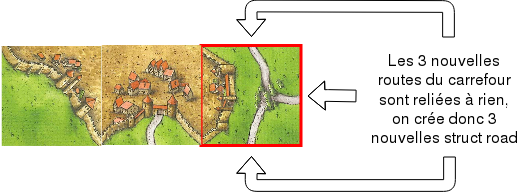
\includegraphics[scale=0.8]{routeModif2.png}
\vspace{0.5cm}

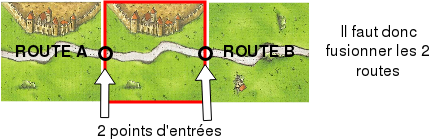
\includegraphics[scale=1]{routeModif1.png}

\vspace{0.5cm}
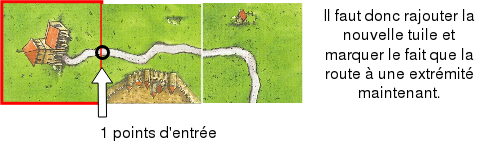
\includegraphics[scale=1]{routeModif3.png}
\vspace{0.5cm}

La mise à jour du score lié aux routes se fait en même temps que celle des routes, si on vient de finir une route lors de l'update on crédite les joueurs majoritaires et on leurs rend leurs pions qui  correspondent à: $points = 2 * len(Route)$



\subsubsection{La mise à jour des villes}
Après avoir rajouté une tuile, on vérifie chaque ville qui la compose :
\begin{itemize}
    \item Soit elle n'est reliée à rien, donc on créé une nouvelle $struct$ $city$ que l'on rajoute à la liste des villes dans la $struct$ $boardgame$.
    \item Soit la ville continue une ou plusieurs villes existantes : il faut donc mettre à jour sa $struct$ $ville$ :
    \begin{itemize}
        \item On regarde donc chaque ville adjacente à notre tuile et on fusionne toutes les $struct$ $city$ qui se recoupent en une nouvelle.
        \item il faut aussi fusionner les champs associés aux villes.
    \end{itemize}
\end{itemize}
\begin{algorithm}[!h]
\caption{Update Town}
\begin{algorithmic} [!h]
\REQUIRE  B : boardgame
\REQUIRE  $T_p $ : tuile piochée
\STATE $Lst_{Ville} \leftarrow Lst_{vide}()$
\STATE $Lst_{Champ_{in\_Ville}} \leftarrow Lst_{vide}()$
\STATE $Lst_{Ville} \leftarrow Extraire\_Ville\_In\_Tuile(T_p) $
\STATE $Lst_{Champ{_in\_Ville}} \leftarrow Extraire\_Champ\_In\_Tuile(T_p) $
\FORALL{$T_i \in Lst_{Ville}$}
\STATE $FusionVille(B,T_i)$
\ENDFOR
\FORALL{$F_i \in Lst_{Champ{_in\_Ville}}$}
\STATE $FusionChamp(B,T_i)$
\ENDFOR
\end{algorithmic}
\end{algorithm}
\newpage 
la complexité est $\mathcal{O}(taille_{max}(F_i) * Nombre\_Champ\_In(B))$.



\vspace{0.5cm}
Exemple de mise en application :

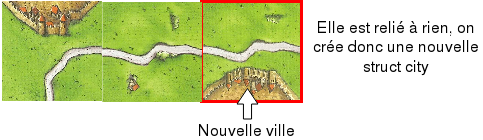
\includegraphics[scale=1]{villeModif2.png}

\vspace{1cm}

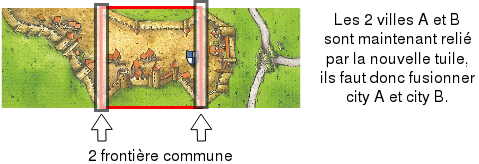
\includegraphics[scale=1]{villeModif1.png}

\vspace{1cm}

La mise à jour du score liée au villes se fait en même temps, si on vient de finir une ville lors de lla mise à jour, on crédite les joueurs majoritaires et on leurs rend leurs pions qui correspondent à: $points = 2 * ( len(Ville) + nombre(bouclier) )$


\subsubsection{La mise à jour des champs}
Après avoir rajouté une tuile, on vérifie chaque champ qui la compose :
\begin{itemize}
    \item Soit il n'est relié à rien et donc on crée une nouvelle $struct$ $field$ que l'on rajoute à la liste des champs dans la $struct$ $boardgame$.
    \item Soit le champ continue un ou plusieurs champs existants : il faut donc mettre à jour les $struct$ $fields$ :
    \begin{itemize}
        \item On regarde donc chaque champ adjacent à notre tuile et on fusionne toutes les $struct$ $fiels$ qui se recoupent en une nouvelle.
    \end{itemize}
\end{itemize}



\begin{algorithm}[!h]
\caption{Update Champ}
\begin{algorithmic} [!h]
\REQUIRE  B : boardgame
\REQUIRE  $T_p $ : tuile piochée
\STATE $Lst_{Champ} \leftarrow Lst_{vide}()$
\STATE $Lst_{Champ} \leftarrow Extraire\_Champ\_In\_Tuile(T_p)$
\FORALL{$F_i \in Lst_{Champ}$}
\STATE $FusionChamp(B,T_i)$
\ENDFOR
\end{algorithmic}
\end{algorithm}

la complexité est $\mathcal{O}(taille_{max}(F_i) * Nombre\_Champ\_In(B))$


\vspace{0.5cm}
Exemple de mise en application :

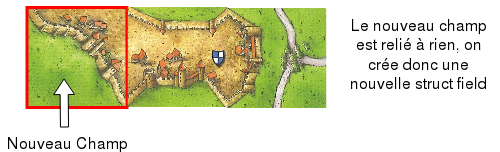
\includegraphics[scale=1]{champModif1.png}

\vspace{1cm}

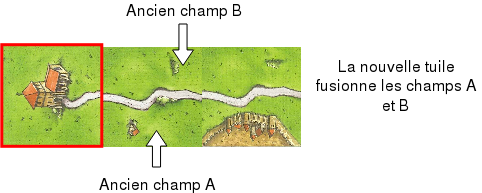
\includegraphics[scale=1]{champModif2.png}

\vspace{1cm}

La mise à jour du score lié au champ ne se fait qu'à la fin, ce qui implique que les pions mis dans un champs ne son pas récupérables.

\subsubsection{La mise à jour des abbayes}

La mise à jour de cette structure est plus simple, il suffit d'incrémenter le nombre de voisins des abbayes autour de la nouvelle tuile et de rajouter les nouvelles abbayes à la liste des abbayes dans le boardgame. 
la complexité est $\mathcal{O}(Nombre\_Abbaye\_In(B))$

La mise à jour du score lié au abbaye se fait en même temps, si on vient de finir une abbaye lors de l'update, on crédite le joueur propriétaire et on lui rend son pion.
Ce qui ce correspond à: $points = 9$

\subsection{Finalisation}

Une fois que toutes les tuiles ont été placées, le jeu est terminé. À cet instant, il faut compter les points fournis par les champs ainsi que les points fournis par les structures non terminées.

La fonction $finalisation$ exécute successivement les fonctions suivantes :
\begin{itemize}
    \item Donner les points aux joueurs possédant une ville non finie.
    \item Donner les points aux joueurs possédant une route non finie.
    \item Accorder les points liés aux champs.
    \item Déclarer le gagnant.
\end{itemize}

Les choses se compliquent avec les champs. En effet, il faut réfléchir en terme de ville. Pour chaque ville finie, le joueur possédant le plus de champs en contact direct avec cette ville gagne trois points. En cas d'égalité, les deux joueurs gagnent trois points (les n joueurs possédant le plus de champ pourplus de précision).\newline

Mais grâce notre $structure$ $city$, rien de plus simple. Les champs en contact avec une ville sont stockés dans la structure. Il suffit donc de voir qui sont les propriétaires de ces champs. \newline

Pour cela, il est nécessaire de regarder chaque champ, de voir à qui il appartient, et de continuer en comptant l'importance des propriétaires (leur nombre de champs en contact avec la ville). Les mêmes règles d'égalités sont appliquées. \newline 


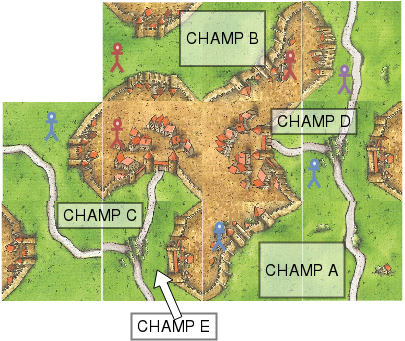
\includegraphics[scale=1]{Comptagepoint.png}

Dans cette situation, quatre champs sont possédés par des joueurs. Ces champs touchent une ville (relativement grosse). De ce fait, le comptage des points se fait de cette manière :
\begin{enumerate}
    \item le joueur rouge possède le champ B
    \item le joueur violet possède le champ D
    \item le joueur bleu possède les champs A et C.
\end{enumerate}

\vspace{0.5cm}

Le joueur bleu possède le plus de champs autour de la ville, il gagne donc trois points, ce qui n'est pas le cas de ses adversaires.
